%%
% 今時jarticleやjbook使ってる人いる?時代はjsarticleかjsbookだよ
% ついでに言うと、uplatexってのはplatexの上位互換、これを使わないなんて旧世代だよね
%
\documentclass[uplatex, report, a4j, 10pt]{jsbook}


%%
% パッケージ群
%
\usepackage{miyazaki-u-paper}   % 宮崎大学工学部の卒論の基本(片山先生作)を、僕がちょっと書き換えちゃった(テヘッ
\usepackage{enumitem}           % enumerate?古い古い
\usepackage[dvipdfmx]{graphicx,hyperref} % 当然dvipdfmなんて使ってないよね
\usepackage[dvipdfmx]{color}    % listingsを使うときにはこれも必須、dvipdfmxを変えちゃうとgraphicxのdvipdfmxも変わるよ
\usepackage{pxjahyper}
\usepackage{listings, jlisting} % コードを埋め込むなら必須
\usepackage{txfonts}            % フォントといえばやっぱりtxfonts、今はnewtxってのもあるらしい
\usepackage{verbatim}           % コメントアウトしてくれる便利なプリアンブルが使える \begin{comment} ... \end{comment}
\usepackage{url}
\usepackage{pdfpages}
\hypersetup{
setpagesize=false,
 bookmarksnumbered=true,%
 bookmarksopen=true,%
 colorlinks=true,%
 linkcolor=black,
 citecolor=black,
}
% \usepackage{easy-todo}
\usepackage[hdivide={21mm, , 21mm}, vdivide={30mm, , 25mm}]{geometry} % スタイルを少し変えたくても\hoffset, \voffsetは使わないでね

% \lstset{language = modelica,
%         basicstyle=\fontsize{9pt}{10.5pt}\ttfamily,
%         backgroundcolor={\color[gray]{.90}},
%         breakindent = 10pt
%         }
%%
% miyazaki-u-paper.sty用設定値
%
\degree{g} % Graduateのg or Masterのm
\figurenumbering{f} % 図目次を付ける場合はt (真) を持つ真偽値を引数に取る関数
\tablenumbering{f} % 表目次を付ける場合はt (真) を持つ真偽値を引数に取る関数
\title{OpenModelicaのシミュレーション結果を\\用いたモータ特性表自動生成ツールの試作}
\author{原田 海人}
\nendo{元} % 年度
\advisor{片山 徹郎 教授} % 修論では無視する
\major{情報システム工学科}




\begin{document}
\maketitle


%
% 本文
% 
\chapter{はじめに}\label{cha:Introduction}
近年、モータは、エアコン・洗濯機・掃除機などの家電製品をはじめ、自動車関係、医療関係など様々な分野に
用いられており\cite{モータ使用製品}、社会に必要不可欠な存在となっている。\\
~はじめに 流れ 案~\\
モータの開発は~で、~の課題がある。それを解決する手段としてシミュレーションがある。
シミュレーションツールの中にOpenModelicaがある。OpenModelicaは~で、~する。
また、結果を画面所にプロットすることで結果を確認できる。
シミュレーションを行った場合、期待通りか結果と比較する。\\
比較する際は、シミュレーション結果から目的のグラフや値を計算等して作成しなければならない。\\
しかし、OpenModelicaではグラフでしか確認できず、具体的な値を取得することが困難である。
そこで、本研究では、モータのシミュレーションをOpenModelicaで行った際のシミュレーション結果の確認にかかる手間を削減することを目的として、
シミュレーション結果のcsvファイルからモータ特性表を自動生成するツールを試作する。\\
% 今回試作したツールで、グラフや値を作成する手間を省くことで、モータ開発の効率化を図る。\\



本論文の構成は、以下の通りである。\\
第2章では、モータ特性表自動生成ツールを試作するために必要となる前提知識について説明する。\\
第3章では、試作したモータ特性表自動生成ツールの構成及び手順について説明する。\\
第4章では、試作したモータ特性表自動生成ツールが正しく動作することを検証する。\\
第5章では、試作したモータ特性表自動生成ツールについて考察する。\\
第6章では、、本論文のまとめとの課題を述べる。\\
\chapter{研究の準備}\label{cha:Preparation}
本章では、本研究で必要となる前提知識を説明する。

\section{モータ作成}\label{motor}
\subsection{仕様書}\label{siyo}
\subsection{シミュレータの役割}\label{simu}

\section{モータ特性表}\label{toku}
\subsection{特性表の種類}\label{syurui}
\subsection{特性表の要素}\label{element}

\section{OpenModelica}\label{OM}

\section{modelica}\label{modelica}



% \section{モータ特性表}\label{win_ap}
% WindowsAPIとは、Windowsプログラミングを行うためにMicrosoftが提供しているAPIのことである[10]。
% APIとはApplication Programming Interfaces の略で、プログラムからソフトウェアを操作するためのインターフェイスのことである[11]。
% WindowsAPIを使用することによって、Windowsアプリを作成するために必要な機能を自ら実装せずにすむので、作業工数を短縮できる[10]。
% 本研究では、ボタンの自動入力などの機能を実装する際に使用した。表2.1に、今回使用する関数を示す。

% \begin{table}[t]
% 	\begin{center}
%   \caption{使用している関数一覧}
%   \begin{tabular}{|l|c|r||r|} \hline
%     関数名 & 説明  \\ \hline \hline
%        GetClientRect & ウィンドウのクライアント領域の座標を取得する。\\ \hline
%        GetDC &ディスプレイデバイスコンテキストのハンドルを取得。\\ \hline
%        CreateDIBSection & DIBとDDB用のビットマップを作成する。 \\ \hline
%        CreateCompatibleDC & メモリデバイスコンテキストのハンドルを取得する。 \\ \hline
% 	   GetForegroundWindow & フォアグラウンドウィンドウのハンドルを取得する。 \\ \hline
%        GetWindowText &フォアグラウンドウィンドウの名前を取得する。\\ \hline
%   \end{tabular}
%   \end{center}
% \end{table}

% \section{Visual Studio}\label{visual_studio}
% Visual Studioとは、MicrosoftがリリースしているWindows環境における統合開発環境のことである[12]。
% 複数のプログラミング言語での開発が可能な開発環境で、Visual Studioを用いることによって、Windowsのクライアントアプリケーションや、
% ハンディターミナルなどのアプリケーション、Webアプリケーションを開発できる。
% 本研究では、テスト支援ツールの概観を作成する際にVisual Studioを用いた。

% \section{Unity}
% Unityとは、ユニティ・テクノロジーズ社が提供する、ゲーム開発フレームワークである。2D、3D、VRなどのゲーム開発で利用されている[13]。
% マルチプラットフォームに対応しており、アセットストアが充実しているため、手軽に高クオリティなゲーム制作ができる。
% 本研究では、作成したテスト支援ツールの適用例で使用するゲームの作成に、このフレームワークを採用する。

% \section{パーティクルフィルター}
% パーティクルフィルター(Particle Filter)とは、確率分布に基づく時系列データの予測手法である[14]。
% パーティクルフィルターでは、現状態から起こりうる多数の次状態を、多数のパーティクルを用いて検出する。
% パーティクルフィルターの基本的な操作手順は、以下の通りである。

% \begin{enumerate}
%   \item リサンプリング : 前フレームでの尤度に従って、パーティクルを撒き直す(追跡対象の周りにパーティクルをばら撒く)。
%   \item 推定 : 等速直線運動や適当な乱数を使い、現フレームにおける追跡対象の位置を推定し、パーティクルを少し動かす。
%   \item 観測 : 現フレームにおける各パーティクルの尤度と重み(正規化)を計算する。つまり、推定の答え合わせをして実際の追跡対象の位置に近いパーティクルの重みを大きくする。
%   			   重みが大きいパーティクルが集中している領域が追跡対象となる。
% \end{enumerate}
% 本研究では、この手法を、キャラクターとオブジェクトの重なり判定に使用する。

% \section{DLL}
% DLL(ダイナミックリンクライブラリ)とは、動的リンクを使ったライブラリである[15]。
% 本研究では、DLLを使うことで、C\#のコードからC++で記述した関数を呼び出す。



\chapter{機能}\label{cha:Function}

本章では、本研究で試作したモータ特性表自動生成ツールの機能について説明する。\\

モータ特性表自動生成ツールは、OpenModelicaでモータのモデルをシミュレーションした時に出力される
csvファイルを読み込み、実行することによって、モータ特性表を生成する。\\

\section{対応するモデル}\label{taioumodel}
今回試作したモータ特性表自動生成ツールでは以下のModelicaモデルのシミュレーション結果に対応する。
\begin{itemize}
	\item モータ単体のモデル
	\item モータ単体のモデルを一つに統一したモデルを使用するモデル
\end{itemize}
なお、今回はモータの中でもブラシ付きDCモータに対応する。\\
以降、上記のモデルについて具体的に説明する。

\subsection{モータ単体のモデル}\label{sec:sub1}
モータ単体のモデルとは、電源部品、抵抗部品、インダクター部品、起電力部品、慣性部品、接地部品の
OpenModelicaでブラシ付きDCモータについてシミュレーションするために、最低限必要となる部品を持つモデルのことである。\\
上記6つの部品が必要な理由は、ブラシ付きDCモータの等価回路\cite{等価回路}をModelicaで表す際に
使用する部品\cite{modelicaシステム本}だからである。\\
ブラシ付きDCモータの等価回路を図\ref{fig:touka}に、モータ単体のモデルを図\ref{fig:tantai_model}に、
モータ単体のモデルをModelicaコードで表したものを図\ref{fig:tantai_modelica}に示す。

\begin{figure}[t]
	\centering
	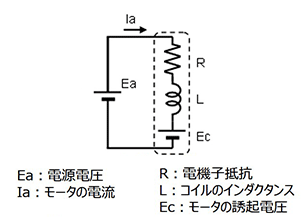
\includegraphics[width=10cm]{./Image/touka.png}
	\caption{等価回路}
	\label{fig:touka}
  \end{figure}

\begin{figure}[t]
  \centering
  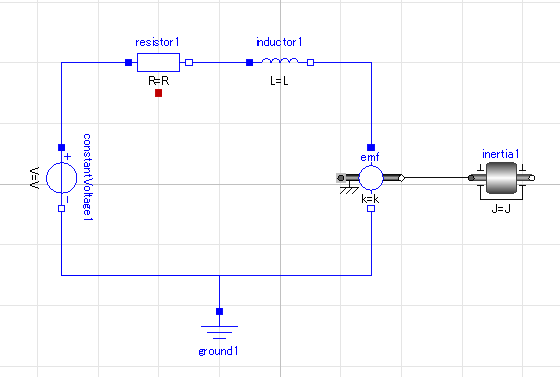
\includegraphics[width=10cm]{./Image/tantai_model.png}
  \caption{モータ単体のモデル}
  \label{fig:tantai_model}
\end{figure}

\begin{figure}[t]
	\centering
	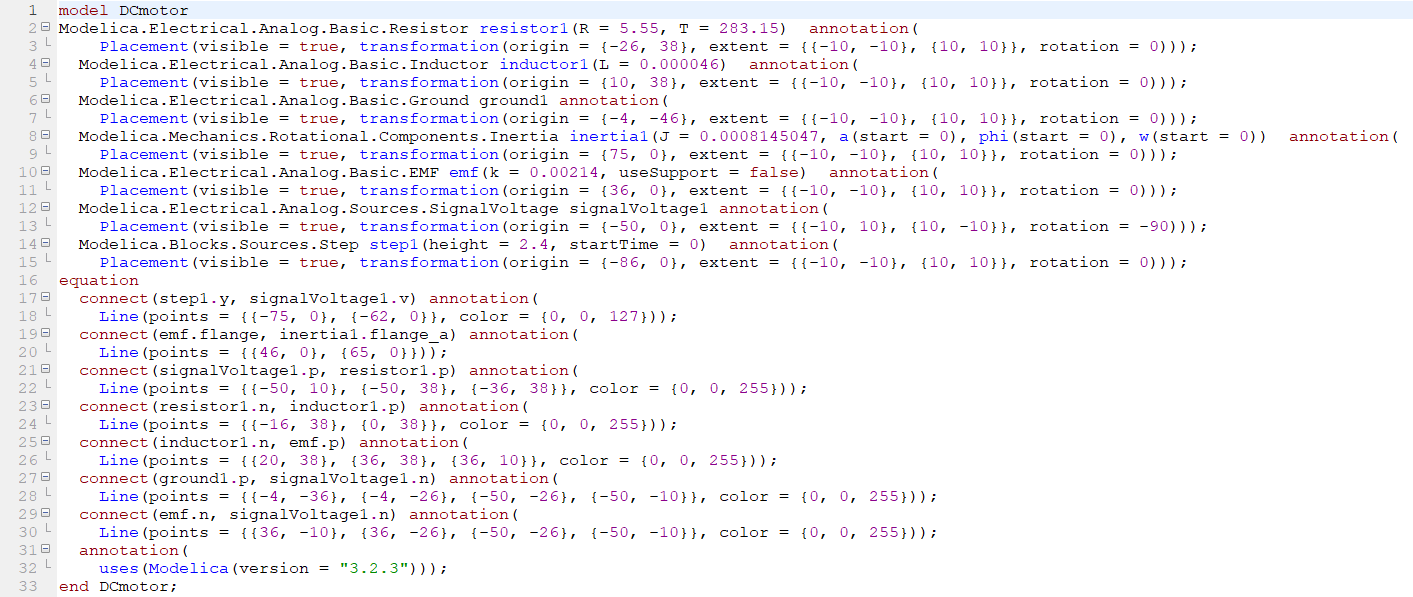
\includegraphics[width=16.5cm,height=8cm]{./Image/tantai_modelica.png}
	\caption{モータ単体のモデルのModelicaコード}
	\label{fig:tantai_modelica}
  \end{figure}

\subsection{モータ単体のモデルをサブシステムとするモデル}\label{sec:sub2}
モータ単体のモデルをサブシステム\cite{modelicaシステム本}(準備に書く?)とするモデルとは、\ref{sec:sub1}節で説明した
モータ単体のモデルを一つのモデルにして、サブシステムとして書いたモデルのことである。


\section{特性表生成}\label{kenkyu_mokuteki}
今回試作したモータ特性表自動生成ツールには次の~~~個の機能がある。

\begin{itemize}
	\item are
	\item sore 
\end{itemize}

\subsection{特性表生成機能}\label{sec:tokusei}
特性表生成機能は、以下の要素を持つモータ特性表を生成する。


\chapter{実装}\label{cha:Implementation}

\section{シミュレーション結果解析機能}\label{kyap_re}

\section{特性表生成機能}\label{gazou_input}

\chapter{適用例}\label{cha:Indication}
本章では、本研究で作成した


\section{モータ単体のモデル}


\section{モータ単体のModelicaモデルをサブシステムとするモデル}

\chapter{考察}\label{cha:Discussion}
本論文では、性能を決定付ける特定の値を確認するためにかかる時間の削減を目的として、モータ特性表自動生成ツールを試作した。

なお、本研究では、シミュレーションの対象として、ブラシ付きDCモータを対象とする。

4章において、本論文で試作したモータ特性表自動生成ツールに、ブラシ付きDCモータのModelicaモデルと、
ブラシ付きDCモータのModelicaモデルをサブシステムとするモデルの2つが出力するcsvファイルを適用した。
その結果、本論文で試作したモータ特性表自動生成ツールが正しく動作することを確認できた。以下に、本論文で試作したモータ特性表自動生成ツールについて考察する。
\section{評価}

\subsection{評価方法}
% \todo{下記のコマンドを書き換える!}
% \newcommand{\mExist}{既存の手法}
% \newcommand{\mExtend}{本研究の手法}
% \newcommand{\mInput}{仕様書}
% \newcommand{\mOutput}{仕様書}

% \mExist{}と、\mExtend{}で、作成(生成)に要した時間の比較検証を行った。
% その結果を、表\ref{tab:time}に示す。

% 対象とした\mInput{}は、\ref{cha:domain}節で用いた コード\ref{fig:vdm_park}である。
% \mOutput{}を作成する時間を計測した。
% 生成する\mOutput{}としては、以下を基準とした。\todo{なにをもって完成かを書く!}
% \begin{enumerate}
%   \item onポイント、offポイント、inポイント、outポイントを出力(記述)する
%   \item onポイント、offポイント、outポイントには、着目条件式も出力(記述)する
%   \item offポイントには、着目変数も出力(記述)する
%   \item 各ポイントには、期待出力と正常系であるかどうかも出力(記述)する
% \end{enumerate}

% 検証に参加したメンバーは本研究室の大学院生\todo{X}人と学部4年生\todo{Y}人であり、
% 普段からソースコードの読み書きを行い、基本的なプログラミングの知識を有している。
% \mInput{}の知識を持たない者も含まれるが、
% 今回の検証に必要な文法は、事前に他の\mInput{}の例を用いてレクチャーした。
% また、\mOutput{}生成についても、事前に他の\mInput{}と\mOutput{}の例を用いてレクチャーした。

% 人手による検証では、
% コード\ref{fig:vdm_park}を印刷した紙を渡し、
% \mInput{}を確認後、
% \mOutput{}を書き始めてから、\mOutput{}を記述し終えるのに要した時間を計測した。
% \todo{なんか}が不正確な場合、間違いを指摘し、
% 被験者が正しい\mOutput{}を記述した時点で時間計測終了とした。
% また、制限時間を\todo{Z}分とし、制限時間を超えた場合、その場で時間計測終了とした。

% \mExtend{}による検証では、
% \todo{計測はじめから終わりの条件と、使ったPCの仕様を書く}
% コマンドライン上での命令操作で、\mExtend{}による\mOutput{}生成を行うのに要した時間を計測した。
% また、実験に用いたコンピュータは、OS:Windows10 Pro、CPU:3.6GHz Intel Core i7、メモリ:16GBである。

% \todo{純粋な、実行時間を書く}
% なお、JavaのSystem.nanoTime\cite{nanotime}メソッドを用いて、
% 命令操作を省いた純粋な\mOutput{}生成処理に\mExtend{}が要した時間を計測した結果、
% \todo{A}秒であった。

% 人手による作成と比較した結果、平均で\todo{B}分程の時間短縮を確認できた。
% 対象にした\mInput{}には、\todo{なにか}独特の文法等は含まれないため、
% \todo{なにか}に対する慣れなどの影響は無視できるものと思われる。
% また、人手による\mOutput{}生成の場合、ヒューマンエラーも見られた。
% \todo{ヒューマンエラーがあったら、具体例を書く}
% 具体的には、offポイントの記述時に、条件式の解釈を間違え、誤った期待出力を記述してしまった。(例:入力(17、 20)の期待出力を``遊園地チケットは割引価格とならない。(妻の年齢 $<$ 16)''と記述した。)
% \mInput{}の規模が拡大すると、人手とコンピュータとの処理効率の差に加えて、
% ヒューマンエラーの有無などにより、\mOutput{}生成に要する時間の差は更に拡大していくと思われる。
% 以上から、\mExtend{}は有用性が向上したと考える。

% % \begin{table}[tp]
% % \centering
% % \caption{コード\ref{fig:vdm_park}の\mOutput{}作成に要した時間の比較}
% % \label{tab:time}
% % \begin{tabular}{cc}
% % \begin{minipage}[c]{0.5\hsize}
% %   \centering
% %   \begin{tabular}{c|c}
% %     被験者  & 時間              \\
% %     \hline
% %     \hline
% %     被験者A & 8m 16s            \\ \hline
% %     被験者B & 10m 23s           \\ \hline
% %     被験者C & 30m(制限時間超過) \\ \hline
% %     被験者D & 24m 04s
% %   \end{tabular}
% % \end{minipage} &
% % \begin{minipage}[c]{0.5\hsize}
% %   \centering
% %   \begin{tabular}{c|c}
% %                  & 時間    \\
% %     \hline
% %     \hline
% %     被験者(平均) & 18m 10s \\ \hline
% %     BWDM         & 0m 15s
% %   \end{tabular}
% % \end{minipage}
% % \end {tabular}
% % \end{table}

本論文で試作したモータ特性表自動生成ツールの有用性を評価するため、本研究室の学部4年生4人に対して、実験を行い、特定の値を確認するためにかかる時間を削減できたかどうかを検証する。
実験には、内容が異なる2つのシミュレーション結果のファイルを用いた。これらのファイルをそれぞれ「ファイルA」、「ファイルB」と定義する。

実験方法は、ケースXとケースYに分けて行う。

ケースXでは、ファイルAに対して、モータ特性表自動生成ツールを使用せず、表計算ソフトを用いて問題に回答してもらう。次に、ファイルBに対して、モータ特性表自動生成ツールを使用して問題に回答してもらう。

ケースYでは、ファイルBに対して、モータ特性表自動生成ツールを使用せず、表計算ソフトを用いて問題に回答してもらう。次に、ファイルAに対して、モータ特性表自動生成ツールを使用して問題に回答してもらう。

ケースXとケースY で出題する問題を、図\ref{fig:mondai}に示す。

この問題を解答するのに要する時間を測定することにより、モータ特性表自動生成ツールを用いることで、特定の値を確認するためにかかる時間を削減できるかどうかを検証する。

被験者4名を2つのグループに分け、片方のグループに「ケースX」の実験を行い、もう片方のグループに「ケースY」の実験を行った。

「ケースX」の実験結果を、表\ref{resultX}に、「ケースY」の実験結果を表\ref{resultY}にそれぞれ示す。

\begin{figure}[t]
	\centering
	\fbox{
	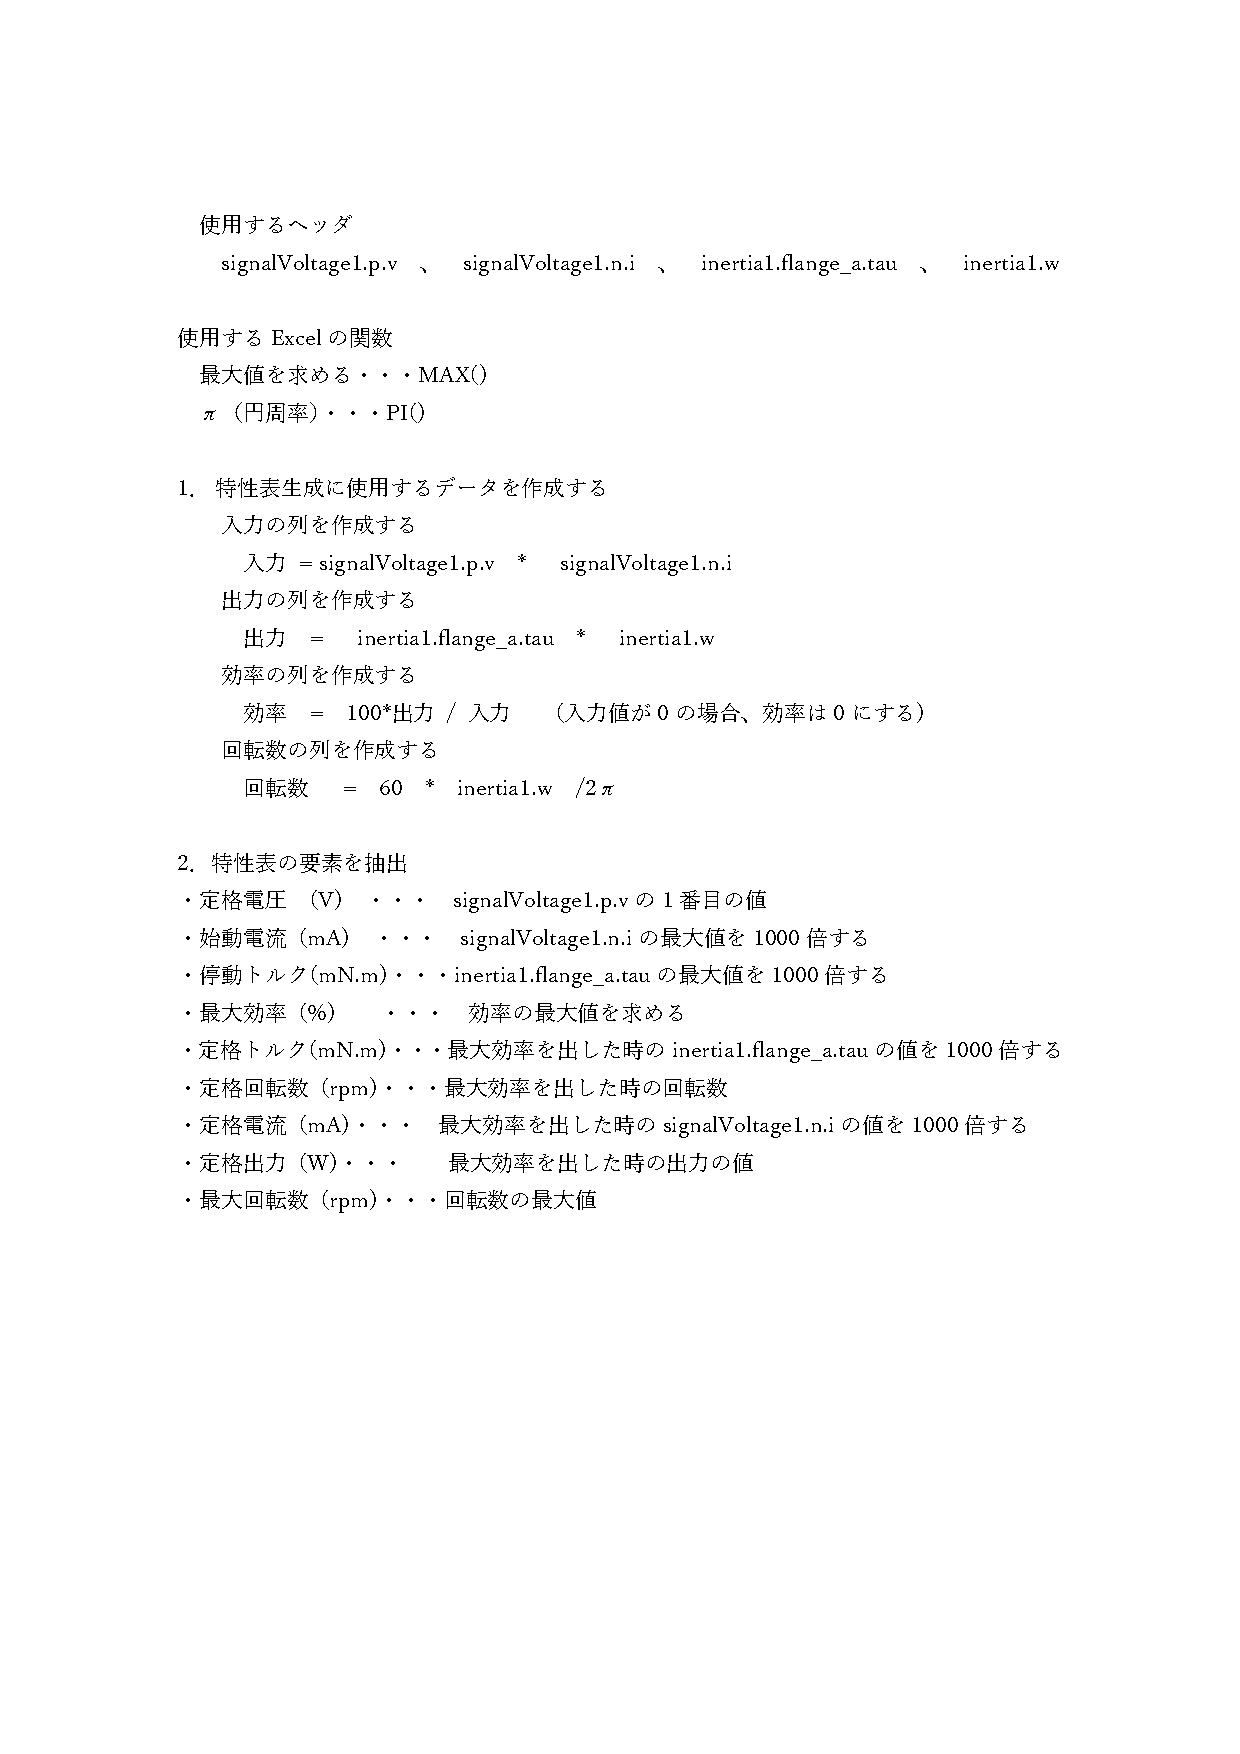
\includegraphics[width=16cm,pagebox=cropbox]{Image/実験方法の説明.pdf}
	}
	\caption{ケースXとケースY で出題する問題}
	\label{fig:mondai}
\end{figure}

\begin{table}[tp]
  \begin{center}
    \caption{ケースXの実験結果}
    \label{resultX}
    \begin{tabular}{c|c|c|c|c|}
    \cline{2-5}
                              & \multicolumn{2}{c|}{ツール未使用} & \multicolumn{2}{c|}{ツール使用} \\ \hline
    \multicolumn{1}{|c||}{被験者} & 回答時間           & 正答率          & 回答時間           & 正答率         \\ \hline\hline
    \multicolumn{1}{|c||}{1}   & 13分5秒           & 56\%         & 57秒           & 100\%         \\ \hline
    \multicolumn{1}{|c||}{2}   & 14分50秒          & 67\%          & 1分20秒          & 100\%         \\ \hline\hline
    \multicolumn{1}{|c||}{平均}   & 13分57.5秒          & 61.5\%          & 1分8.5秒          & 100\%         \\ \hline
    \end{tabular}
  \end{center}
\end{table}

\begin{table}[tp]
  \begin{center}
    \caption{ケースYの実験結果}
    \label{resultY}
    \begin{tabular}{c|c|c|c|c|}
    \cline{2-5}
                              & \multicolumn{2}{c|}{ツール未使用} & \multicolumn{2}{c|}{ツール使用} \\ \hline
    \multicolumn{1}{|c||}{被験者} & 回答時間           & 正答率          & 回答時間           & 正答率         \\ \hline\hline
    \multicolumn{1}{|c||}{3}   & 21分35秒           & 67\%         & 1分10秒           & 100\%         \\ \hline
    \multicolumn{1}{|c||}{4}   & 18分6秒          & 100\%          & 1分58秒          & 89\%         \\ \hline\hline
    \multicolumn{1}{|c||}{平均}   & 19分50.5秒          & 83.5\%          & 1分34秒          & 94.5\%         \\ \hline
    \end{tabular}
  \end{center}
\end{table}

「ケースX」の実験結果から、モータ特性表自動生成ツールを用いない場合の解答時間の平均は「13分57.5秒」である。また、正答率の平均は「61.5\%」である。
一方、モータ特性表自動生成ツールを用いた場合の解答時間の平均は「1分8.5秒」である。また、正答率の平均は「100\%」である。

この結果から、「ケースX」の実験においてモータ特性表自動生成ツールを用いた場合、解答時間の平均は用いなかった場合に比べて「91.8」\%削減できた。
また、モータ特性表自動生成ツールを用いた場合の方が、用いなかった場合に比べて正答率が高いことが示せた。

「ケースY」の実験結果から、モータ特性表自動生成ツールを用いない場合の解答時間の平均は「19分50.5秒」である。また、正答率の平均は「83.5\%」である。
一方、モータ特性表自動生成ツールを用いた場合の解答時間の平均は「1分34秒」である。また、正答率の平均は「94.5\%」である。

この結果から、「ケースY」の実験においてモータ特性表自動生成ツールを用いた場合、解答時間の平均は用いなかった場合に比べて「92.1」\%削減できた。
また、モータ特性表自動生成ツールを用いた場合の方が、用いなかった場合に比べて正答率が高いことが示せた。


これらの結果により、モータ特性表自動生成ツールを用いることで、特定の値を確認するためにかかる時間を削減できることを確認した。
また、モータ特性表自動生成ツールを用いることで、正答率が上がったことを確認できた。正答率が上がった理由として、モータ特性表自動生成ツールを用いることにより、人手によるミスを削減できたことが考えられる。
具体的には、モータ特性表自動生成ツールを用いない場合、手動で表計算ソフトから特定の値を抽出し、計算を行う必要があるため、この過程においてミスが発生する可能性が高まったことが考えられる。
一方、モータ特性表自動生成ツールを用いた場合、ツールが自動で特性表を生成し、提示することにより、人手によるミスが発生する可能性を削減できたことが考えられる。

以上の結果により、モータ特性表自動生成ツールの有用性があることを示せた。また、モータ特性表自動生成ツールを用いることで、特定の値を確認する際に生じるミスを削減できることが確認できた。


\subsection{結果}
本論文で試作したモータ特性表自動生成ツールは、

\section{関連研究}
関連研究について考察する。

\subsection{MATLABとの比較}
モデルベースシステム開発で使用されるツールとして、OpenModelicaの他に、MATLABがある。
MATLABはMathWorks社が開発する科学技術計算用のプログラミング言語である。
MATLABは、制御システム、信号処理、ディープラーニングなど幅広い分野の科学技術計算ができる。
また、ブロック線図シミュレータであるSimulinkと連携させることで、モータのモデル化、シミュレーション、グラフの描画ができる。
しかし、モータの性能を決定づける値の算出や、グラフの描画はできるが、モータの特性表の自動生成はできない。
一方、本研究で試作したモータ特性表自動生成ツールは、OpenModelicaのシミュレーション結果から、モータ特性表を自動生成できる。
このため、特性表と特性グラフをまとめたモータ特性表を自動生成できることが試作したツールの利点といえる。


\subsection{JMAG-Express Onlineとの比較}
\begin{table}[t]
	\centering
	\caption{本研究で試作したモータ特性表自動生成ツールにおけるモータ特性表出力までの実行時間}
	\begin{tabular}{|c|c|} \hline
	  ファイルサイズ(KB) & 実行時間(s)\\ \hline \hline
	  37 & 0.884 \\ \hline
	  47 &  0.978\\ \hline
	  2,909 &  1.024 \\ \hline
	  3,569 & 1.025 \\ \hline
	  5,496 &  1.078\\ \hline
	  71,987 &  3.329 \\ \hline
	\end{tabular}
	\label{tab:executionTime}
  \end{table}

パラメータベースのモータ設計支援ツールとして、JSOL社が開発するJMAG-Express Online(以下JMAG)がある\cite{jmag}。
JMAGは、形状テンプレート、材料、巻線および駆動条件のパラメータを入力することで、
モータ特性表(特性表と特性グラフ)を生成することができる。
さらに、モータ特性表に出力する基本特性(トルク、回転数など)は1秒程度で計算できる。
しかし、パラメータベースのモータ設計支援ツールであるため、
モデルベースシステム開発の利点である柔軟な開発が、JMAGを利用できない。
一方、本研究で試作したモータ特性表自動生成ツールは、OpenModelicaのシミュレーション結果から、
モータ特性表を自動生成できる。
ここで、本研究で試作したモータ特性表自動生成ツールにおけるモータ特性表出力までの実行時間を、表\ref{tab:executionTime}にそれぞれ示す。
表\ref{tab:executionTime}が示すように、試作したツールも1秒程度でモータ特性表に出力する基本特性を計算できるため、JMAGと同程度の時間で、モータ特性表を生成できる。
このため、モータをモデルベースシステム開発手法で開発する際に、試作したツールを用いてモータの性能を確認できることが、試作したツールの利点といえる。

\section{ツールの問題点}

以下に、今回作成したモータ特性表自動生成ツールの問題点を示す。

\begin{itemize}
	\item 対象とするモータのモデルが1種類しかない\\
      本論文で試作したモータ特性表自動生成ツールが対象とするのはブラシ付きDCモータである。しかし、ブラシレスモータやACモータなどには対応していない。
      そのため、それらを用いた回路のシミュレーション結果からモータ特性表を作成できない。
		  この問題点は、新たに対象とするモータのcsvファイルを解析し、特性表の要素を算出できるようにすることで、解決できると考える。

  \item 特性表の要素をユーザが変更できない\\
        本論文で試作したモータ特性表自動生成ツールが生成する特性表は、12個の要素を持つ。
        しかし、ユーザがこの要素を変更することはできない。
        この問題点は、ユーザが特性表の要素を設定できるようにすることで、解決できると考える。

  \item 特性グラフを出力形式をユーザが指定できない\\
        本論文で試作したモータ特性表自動生成ツールは、4つの特性グラフを個別に出力する。
        しかし、特性グラフは1つのグラフに複数の要素を表示することで、グラフの比較を行いやすくなる。
        そのため、特性グラフの出力形式をユーザが指定できるようにすることで、グラフの比較がしやすくなり、 本論文で試作したモータ特性表自動生成ツールの有用性が向上すると考える。


\end{itemize}








\chapter{おわりに}\label{cha:Conclusion}


以下に、今後の課題を示す。





%% listings-modelica.cfg
%% Copyright 2014 Martin Sjoelund, Dietmar Winkler
%
% This work may be distributed and/or modified under the
% conditions of the LaTeX Project Public License, either version 1.3
% of this license or (at your option) any later version.
% The latest version of this license is in
%   http://www.latex-project.org/lppl.txt
% and version 1.3 or later is part of all distributions of LaTeX
% version 2005/12/01 or later.
%
% This work has the LPPL maintenance status `maintained'.
%
% The Current Maintainer of this work is Dietmar Winkler
%
% Code repository https://github.com/modelica-tools/listings-modelica
%
% This work consists of the file listings-modelica.cfg

\lstdefinelanguage{modelica}
{
  morekeywords=[1]{
    algorithm,and,annotation,as,assert,block,break,case,class,connect,connector,
    constant,constrainedby,der,discrete,each,else,elseif,elsewhen,encapsulated,
    end,enumeration,equality,equation,expandable,extends,external,failure,final,
    flow,for,function,guard,if,import,in,initial,inner,input,List,local,loop,
    match,matchcontinue,model,not,operator,Option,or,outer,output,package,parameter,
    partial,protected,public,record,redeclare,replaceable,return,stream,
    subtypeof,then,Tuple,type,uniontype,when,while},
  morekeywords=[2]{true, false},
  % Do not make true,false keywords because fn(true,x, false ) shows up as fn(true,x, *false*)
  morekeywords=[3]{optimization,constraint}, % Optimica keywords
  morekeywords=[4]{objective,startTime,finalTime,initialGuess},
  sensitive=true,
  comment=[l]//,
  morecomment=[s]{/*}{*/},
  alsodigit={.,-},
  morestring=[b]',
  morestring=[b]",
}[keywords,comments,strings]

\definecolor{keywordcolor1}{rgb}{0,0,.4}
\definecolor{keywordcolor2}{rgb}{.90,0,0}
\definecolor{keywordcolor3}{rgb}{.4,0,.8}
\definecolor{keywordcolor4}{rgb}{0.5,0,0.5}
\definecolor{stringcolor}{rgb}{0.133,0.545,0.133}
% \definecolor{listingbgcolor}{rgb}{0.95,0.95,0.95}

\lstset{
  breaklines=true,
  language=modelica,
  basicstyle=\ttfamily,
  keywordstyle=[1]\color{keywordcolor1}\bfseries,
  keywordstyle=[2]\color{keywordcolor2},
  keywordstyle=[3]\color{keywordcolor3}\bfseries,
  keywordstyle=[4]\color{keywordcolor4},
  stringstyle=\color{stringcolor},
%  backgroundcolor=\color{listingbgcolor},
  framexleftmargin=5pt,
  xleftmargin=5pt,
  xrightmargin=5pt,
  showstringspaces=false
}

\newcommand{\code}[1]{\lstinline|#1|}
\newcommand{\modelica}[1]{\lstinline[language=modelica]|#1|}

%%
% 謝辞
%
\acknowledgment


%%
% 参考文献
%

\bibliography{bibtex} %bibファイルの.bibの前の部分
\bibliographystyle{junsrt} %引用された順番に出力
% \newpage
% \listoftodos
\end{document}